\documentclass[a4paper,11.5pt,UTF8]{ctexart}
\usepackage{a4}
\usepackage{amsmath, amssymb, amsthm, graphicx, xspace,array,url}
\usepackage{setspace}
\usepackage{float}
\usepackage{listings,color,xcolor,fontspec}

\CTEXsetup[format={\Large\bfseries}]{section}

\lstset{
	columns=fixed,       
	numbers=left,                                        % 在左侧显示行号
	numberstyle=\tiny\color{gray},                       % 设定行号格式
	frame=none,                                          % 不显示背景边框
	backgroundcolor=\color[RGB]{245,245,244},            % 设定背景颜色
	keywordstyle=\color[RGB]{40,40,255},                 % 设定关键字颜色
	numberstyle=\footnotesize\color{darkgray},           
	commentstyle=\it\color[RGB]{0,96,96},                % 设置代码注释的格式
	stringstyle=\rmfamily\slshape\color[RGB]{128,0,0},   % 设置字符串格式
	showstringspaces=false,                              % 不显示字符串中的空格
	language=c++,                                        % 设置语言
}

\title{Homework 3}
\author{张卓涵 3190101161}
\usepackage[a4paper,left=20mm,right=20mm,top=30mm,bottom=20mm]{geometry}

\newtheorem{example}{\hspace{2em}例}{}
\newtheorem{remark}{\hspace{2em}注}{}
\newtheorem{thm}{\hspace{2em}定理}{}
\newtheorem{lemma}{\hspace{2em}引理}{}

\begin{document}
\begin{figure}[t]
\begin{minipage}[h]{0.25\linewidth}
	
\includegraphics[width=4.0cm]{ZJU2.jpeg}
\end{minipage}
\hfill
\begin{minipage}[h]{.7\linewidth}
	\begin{flushright}
			\Large{数值分析
				\vspace{3mm}	\\
				   2021 冬
				\vspace{3mm}	\\
				   张卓涵 \hspace{3mm}3190101161}
	\end{flushright}
\end{minipage}
\rule{\linewidth}{0.1em}
\end{figure}
\begin{center}
	\huge{\textbf{Homework 3}}
\end{center}

\begin{large}
	
\section{Theoretical Questions}
\subsection{Assignment.\uppercase\expandafter{\romannumeral1}}
$$ p(0)=0,\quad p(1)=1,\quad p'(1)=-3,\quad p''(1)=6 $$
\par 构造差分表为:
\begin{center}
	\begin{tabular}{c|c c c c}
		0 & 0 & & & \\
		\hline
		1 & 1 & 1 &  & \\
		\hline
		1 & 1 & -3 & -4 & \\
		\hline
		1 & 1 & -3 & 3 & 7
	\end{tabular}
\end{center}
$$ p(x)=x-4x(x-1)+7x(x-1)^2=7x^3-18x^2+12x $$
\par 而$s''(0)\neq 0$,因此$p(x)$不是自然三次样条。

\subsection{Assignment.\uppercase\expandafter{\romannumeral2}}
\begin{itemize}
	\item[(a)] 因为$s\in \mathbb{S} ^1_2$,在构造$p_1(x)$时,只有$p_1(x_1)=f_1$和$p_1(x_2)=f_2$两个条件,而想构造2次多项式$p_1(x)$,还需要1个条件。
	\item[(b)] 通过构造差分表可以求出:
	$$p_i(x)=f_i+m_i(x-x_i)+\frac{f_{i+1}-f_i+m_i(x_{i+1}-x_i)}{(x_{i+1}-x_i)^2}(x-x_i)^2$$
	\item[(c)] 通过差分表构造出$p_i(x)$为:
	$$p_i(x)=f_i+m_i(x-x_i)+\frac{f[x_i,x_{i+1}]-m_i}{x_{i+1}-x_i}(x-x_i)^2$$
	由$p'_{i-1}(x_i)=p'_i(x_i)$化简得到:
	$$m_{i-1}+m_i=2f[x_{i-1},x_i],\quad i=2,3,\cdots,n$$
	联立后求解线性方程组即可求出$m_2,m_3,\cdots,m_{n-1}$.
\end{itemize}

\subsection{Assignment.\uppercase\expandafter{\romannumeral3}}
由Lemma4.3和Lemma4.5有以下二式:
\begin{align*}
	\frac{1}{2}s'_1(-1)+2s'_1(0)+\frac{1}{2}s'_2(1) & =\frac{3}{2}\left[s_2(1)-1-c\right]+\frac{3}{2}c \\
	\frac{1}{2}s''_1(-1)+2s''_1(0)+\frac{1}{2}s''_2(1) & = 3\left(s_2(1)-1-c\right)
\end{align*}
得出:$s_2(1)=6c+1,\ s'_2(1)=6c$,结合$s_2(0)=s_1(0)=1+c,\ s''_2(1)=0$得:
$$s_2(x)=1+c+5cx+cx(x-1)-cx(x-1)^2=-cx^3+3cx^2+3cx+c+1$$
若$s(1)=-1$,则$c=-\frac{1}{3}$.

\subsection{Assignment.\uppercase\expandafter{\romannumeral4}}
\begin{itemize}
	\item[(a)] 首先有$f_1=0,\ f_2=1,\ f_3=0$,接着由$M_1=M_3=0$求出$M_2=-3$.于是由Lemma4.5构造出$s(x)$为:
	\begin{equation*}
	s(x)=
		\begin{cases}
			-\frac{1}{2}x^3-\frac{3}{2}x^2+1& x\in [-1,0] \\
			\frac{1}{2}x^3-\frac{3}{2}x^2+1& x\in [0,1]
		\end{cases} 
	\end{equation*}
	\item[(b)] 首先我们有:
	$$\int_{-1}^{1}\left[s''(x)\right]^2dx=6$$
	\begin{itemize}
		\item[(i)] 此时,$g(x)=x+1-x(x+1)=-x^2+1$,那么
		$\int_{-1}^{1}\left[g''(x)\right]^2dx=8$,故而有
		$$\int_{-1}^{1}\left[s''(x)\right]^2dx < \int_{-1}^{1}\left[g''(x)\right]^2dx$$
		\item[(ii)] 此时,$g(x)=f(x)=cos(\frac{\pi}{2}x)$,那么$\int_{-1}^{1}\left[g''(x)\right]^2dx=\frac{\pi^4}{16}>6$,因此
		$$\int_{-1}^{1}\left[s''(x)\right]^2dx < \int_{-1}^{1}\left[g''(x)\right]^2dx$$
	\end{itemize}
\end{itemize}

\subsection{Assignment.\uppercase\expandafter{\romannumeral5}}
\begin{itemize}
	\item[(a)] \begin{align*}
		B_i^2(x) &= \frac{x-t_{i-1}}{t_{i+n}-t_{i-1}}\hat{B_i}(x)+\frac{t_{i+n+1}-x}{t_{i+n+1}-t_{i}}\hat{B}_{i+1}(x) \\
		&= \begin{cases}
			\frac{(x-t_{i-1})^2}{(t_{i+1}-t_{i-1})(t_i-t_{i-1})} & x\in(t_{i-1},t_i] \\
			\frac{(x-t_{i-1})(t_{i+1}-x)}{(t_{i+1}-t_{i-1})(t_{i+1}-t_{i})}+\frac{(t_{i+2}-x)(x-t_{i})}{(t_{i+2}-t_{i})(t_{i+1}-t_{i})} & x\in (t_i,t_{i+1}] \\
			\frac{(t_{i+2}-x)^2}{(t_{i+2}-t_{i})(t_{i+2}-t_{i+1})} & x\in (t_{i+1},t_{i+2}]\\ 
			0 & otherwise
		\end{cases}
	\end{align*}
	\item[(b)] 由Thm4.35:
	$$\frac{d}{dx}B_i^2(x)=\frac{2B_i^1(x)}{t_{i+1}-t_{i-1}}-\frac{2B_{i+1}^1(x)}{t_{i+2}-t_{i}}$$ 因为右式两项都在$t_i,t_{i+1}$上连续,则$\frac{d}{dx}B_i^2(x)$在$t_i,t_{i+1}$上连续。
	\item[(c)] 当$x\in (t_{i-1},t_i]$时,上式右端前半项不为0,后半项为0,则$x$不是零点。同理,$x\in(t_{i+1},t_{i+2}]$时也是如此。则$x^*\in[t_i,t_{i+1})$,且
	$$x^*=\frac{t_{i+1}t_{i+2}-t_it_{i-1}}{t_{i+2}+t_{i+1}-t_i-t_{i-1}}$$
	\item[(d)] 首先$B_i^2(x)\geqslant 0$,又因为$\frac{d}{dx}B_i^2(x)$只有$x^*$一个零点,且$x<x^*$时$B_i^2(x)$递增,$x>x^*$时$B_i^2(x)$递减,则$$\max B_i^2(x)=B_i^2(x^*)<1$$
	于是,$B_i^2(x)\in [0,1)$.
	\item[(e)] 绘制$B_1^2(x)$图像如下:
	\begin{figure}[b]
		\centering
		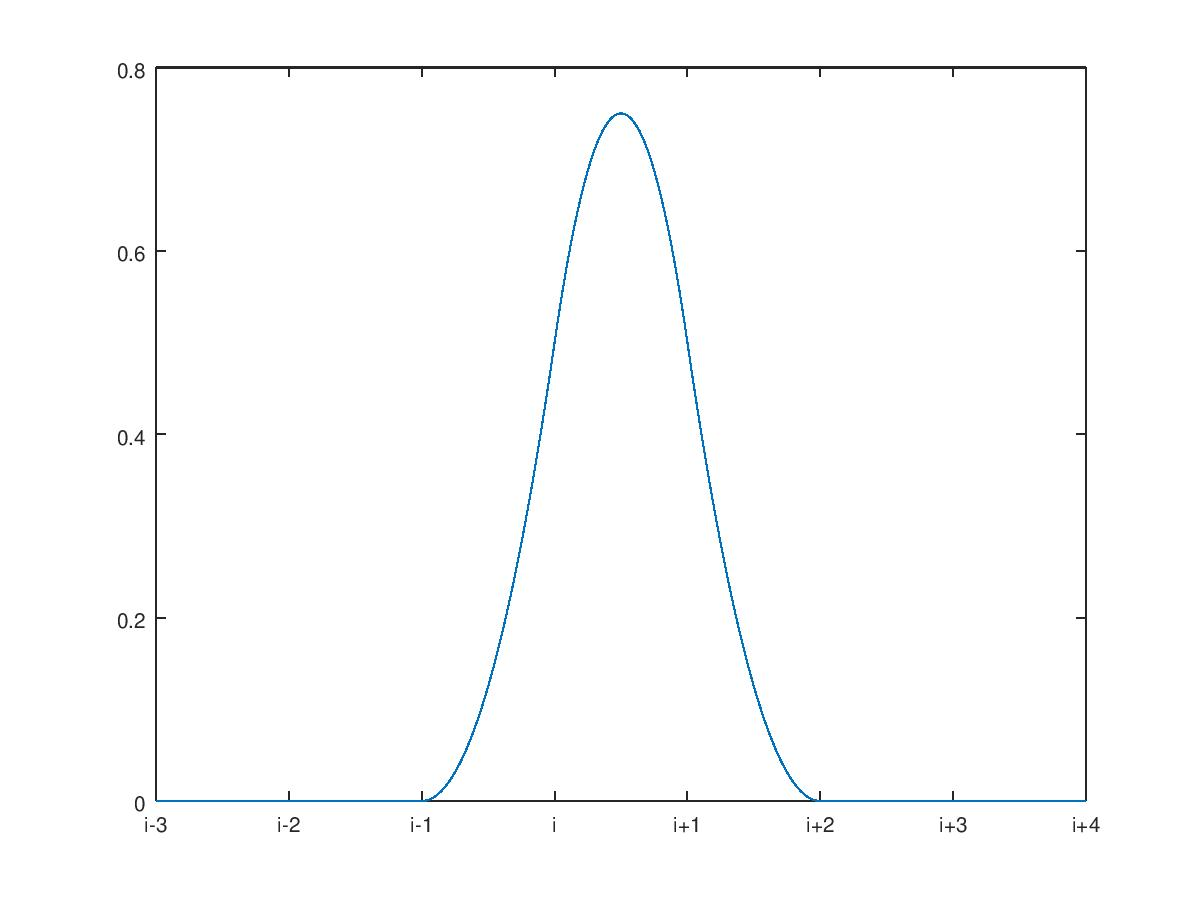
\includegraphics[width=15cm,height=7.4cm]{plot.jpg}
	\end{figure}
\end{itemize}

\subsection{Assignment.\uppercase\expandafter{\romannumeral6}}
\begin{align*}
	& (t_{i+2}-t-{i-1})[t_{i-1},t_i,t_{i+1},t_{i+2}](t-x)_+^2 \\
	= &  \frac{\frac{(t_{i+1}-x)_+^2-(t_i-x)_+^2}{t_{i+1}-t_i}-\frac{(t_i-x)_+^2-(t_{i-1}-x)_+^2}{t_i-t_{i-1}}}{t_{i+1}-t_{i-1}}-\frac{\frac{(t_{i+2}-x)_+^2-(t_{i+1}-x)_+^2}{t_{i+2}-t_{i+1}}-\frac{(t_{i+1}-x)_+^2-(t_i-x)_+^2}{t_{i+1}-t_i}}{t_{i+2}-t_i} \\
	= & \begin{cases}
		\frac{(x-t_{i-1})^2}{(t_{i+1}-t_{i-1})(t_i-t_{i-1})} & x\in(t_{i-1},t_i] \\
		\frac{(x-t_{i-1})(t_{i+1}-x)}{(t_{i+1}-t_{i-1})(t_{i+1}-t_{i})}+\frac{(t_{i+2}-x)(x-t_{i})}{(t_{i+2}-t_{i})(t_{i+1}-t_{i})} & x\in (t_i,t_{i+1}] \\
		\frac{(t_{i+2}-x)^2}{(t_{i+2}-t_{i})(t_{i+2}-t_{i+1})} & x\in (t_{i+1},t_{i+2}]\\ 
		0 & otherwise 
	\end{cases} \\
	= & B_i^2(x)
\end{align*}

\subsection{Assignment.\uppercase\expandafter{\romannumeral7}}
\par 由Thm4.35:对$\forall n\geqslant 1$,
\begin{align*}
	0&=B_{i}^{n+1}(t_{i+n+1})-B_{i}^{n+1}(t_{i-1})=\int_{t_{i-1}}^{t_{i+n+1}}\left[ \frac{d}{dx}B_i^{n+1}(x) \right]dx \\
	&=\frac{n}{t_{i+n}-t_{i-1}}\int_{t_{i-1}}^{t_{i+n+1}}B_i^n(x)dx - \frac{n}{t_{i+n+1}-t_i}\int_{t_{i-1}}^{t_{i+n+1}}B_{i+1}^n(x)dx \quad\cdots (*)
\end{align*}
注意到,$x\in[t_{i+n},t_{i+n+1}]$时,$B_i^n(x)=0$,且$x\in[t_{i-1},t_i]$时,$B_{i+1}^n(x)=0$.因此,
\begin{align*}
	&(*)=\frac{n}{t_{i+n}-t_{i-1}}\int_{t_{i-1}}^{t_{i+n}}B_i^n(x)dx - \frac{n}{t_{i+n+1}-t_i}\int_{t_{i}}^{t_{i+n+1}}B_{i+1}^n(x)dx =0 \\
	\implies & \frac{1}{t_{i+n}-t_{i-1}}\int_{t_{i-1}}^{t_{i+n}}B_i^n(x)dx = \frac{1}{t_{i+n+1}-t_i}\int_{t_{i}}^{t_{i+n+1}}B_{i+1}^n(x)dx
\end{align*}
于是,$B_i^n(x)$与$B_{i+1}^n(x)$的scaled integral相等,即$B_i^n(x)$的scaled integral与i无关。


\subsection{Assignment.\uppercase\expandafter{\romannumeral8}}
\begin{itemize}
	\item[(a)] 构造差分表:
	\begin{center}
		\begin{tabular}{c|c c c}
			$x_i$ & $x_i^4$ & & \\
			\hline
			$x_{i+1}$ & $x_{i+1}^4$ & $(x_{i+1}+x_i)(x_{i+1}^2+x_i^2)$ & \\
			\hline
			$x_{i+2}$ & $x_{i+2}^4$ & $(x_{i+2}+x_{i+1})(x_{i+2}^2+x_{i+1}^2)$ & $[x_i,x_{i+1},x_{i+2}]x^4$ 
		\end{tabular}
	\end{center}
	于是推出:
	\begin{align*}
		[x_i,x_{i+1},x_{i+2}]x^4 &= \frac{(x_{i+2}+x_{i+1})(x_{i+2}^2+x_{i+1}^2)-(x_{i+1}+x_i)(x_{i+1}^2+x_i^2)}{x_{i+2}-x_i} \\
		&=\tau_2(x_i,x_{i+1},x_{i+2})
	\end{align*}
	\item[(b)] 由Lemma4.46:
	\begin{align*}
		&(x_{n+1}-x_1)\tau_k(x_1,\cdots,x_n,x_{n+1}) \\
		=& \tau_{k+1}(x_1,\cdots,x_n,x_{n+1})-\tau_k(x_1,\cdots,x_n)-x_1\tau_k(x_1,\cdots,x_n,x_{n+1}) \\
		=& \tau_{k+1}(x_1,\cdots,x_n,x_{n+1})+x_1\tau_k(x_1,\cdots,x_n,x_{n+1})-\tau_{k+1}(x_1,\cdots,x_n)-x_1\tau_k(x_1,\cdots,x_n,x_{n+1}) \\
		=& \tau_{k+1}(x_2,\cdots,x_n,x_{n+1})-\tau_{k+1}(x_1,\cdots,x_n)
	\end{align*}
	接着采用归纳法,对$n=0$,必然有$$\tau_m(x_i)=[x_i]x^m$$
	现在假设待证式对非负整数$n<m$成立,那么上面的推导表明:
	\begin{align*}
		& \tau_{m-n-1}(x_i,\cdots,x_{i+n+1}) \\
		=& \frac{\tau_{m-n}(x_{i+1},\cdots,x_{i+n+1})-\tau_{m-n}(x_i,\cdots,x_{i+n})}{x_{i+n+1}-x_i} \\
		=& \frac{[x_{i+1},\cdots,x_{i+n+1}]x^m-[x_i,\cdots,x_{i+n}]x^m}{x_{i+n+1}-x_{i}} \\
		=& [x_i,\cdots,x_{i+n+1}]x^m
	\end{align*}
	由归纳法,证毕。
\end{itemize}

\section{Programming}
\subsection{Assignment.B}
\begin{itemize}
	\item[(1)] \par 程序输出结果绘制图像如下:
	\begin{figure}[H]
		\centering
		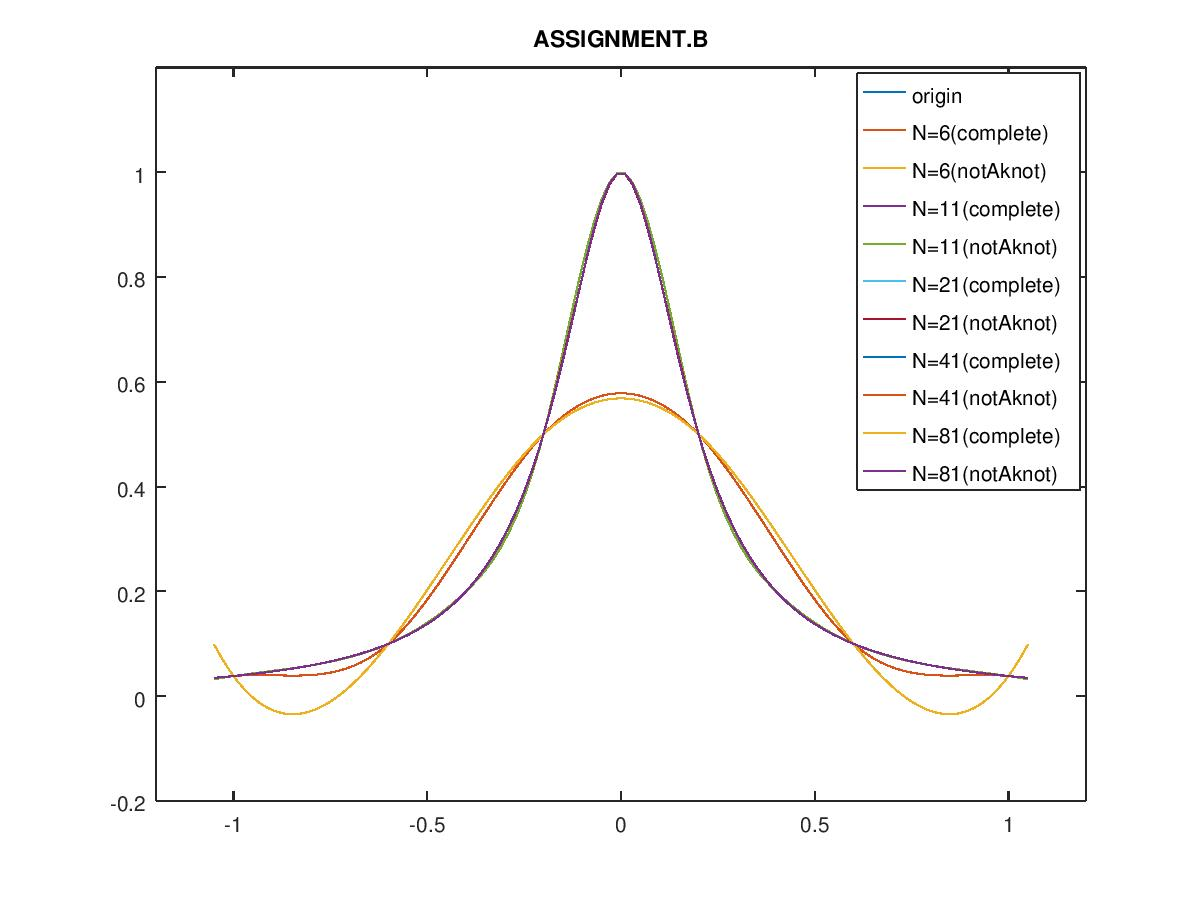
\includegraphics[width=0.65\textwidth]{../plot/figure/figure_B.jpg}
	\end{figure}
	\item[(2)] 相应的误差向量的max-norm为:
	\begin{lstlisting}
	When n = 10:
	Error for complete cubic spline: 0.0205289
	Error for notAknot cubic spline: 0.0205334
	When n = 20:
	Error for complete cubic spline: 0.00316894
	Error for notAknot cubic spline: 0.00316894
	When n = 40:
	Error for complete cubic spline: 0.00012413
	Error for notAknot cubic spline: 0.00012413
	When n = 80:
	Error for complete cubic spline: 7.04042e-06
	Error for notAknot cubic spline: 7.04042e-06
	\end{lstlisting}
	可以看到收敛速度几乎一致。
\end{itemize}

\subsection{Assignment.C \& D}
\begin{itemize}
	\item[(1)] 习题C的输出图像如下:
	\begin{figure}[H]
		\centering
		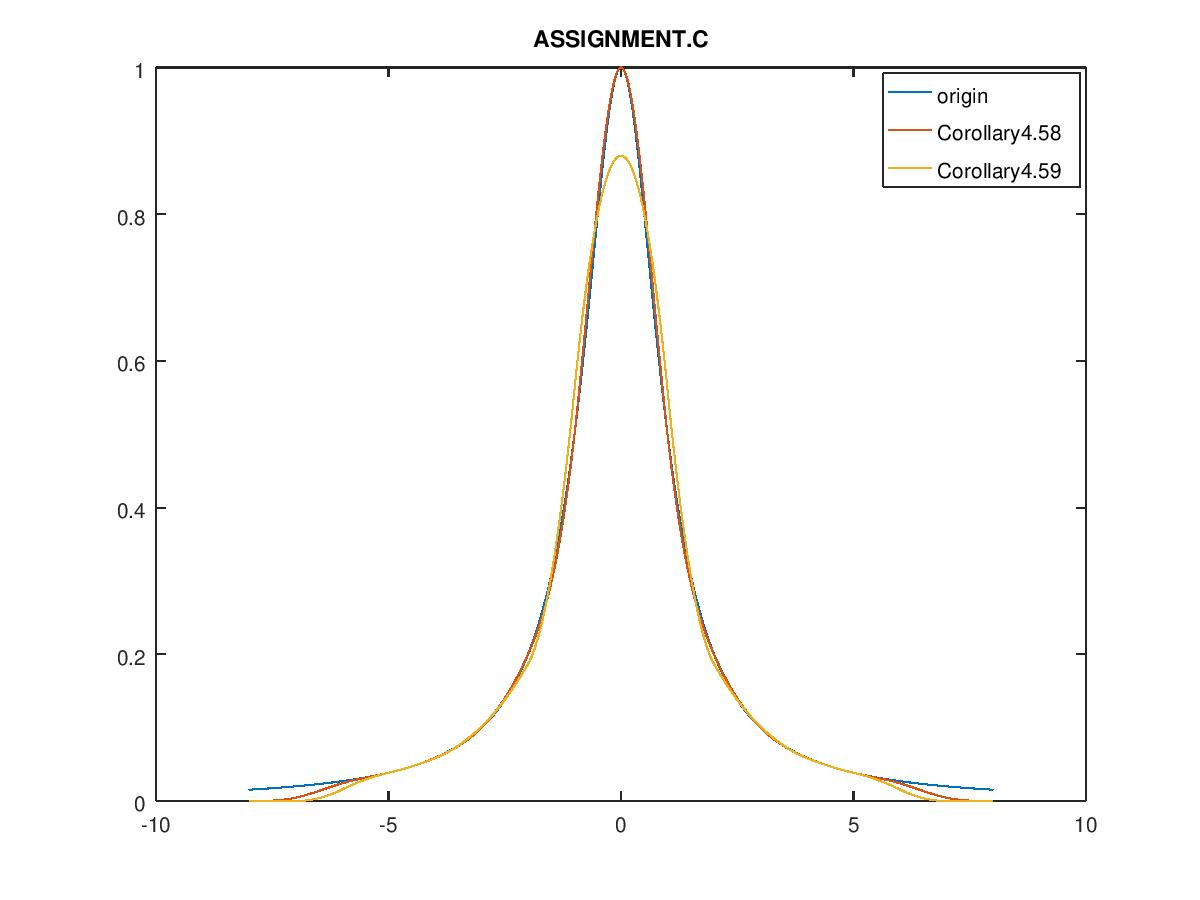
\includegraphics[width=0.65\textwidth]{../plot/figure/figure_C.jpg}
	\end{figure}
	\item[(2)] 习题D的输出结果见于./output/exercise\_CD.txt,有些误差非常接近机器精度是因为,这些点本身就是选取的“knots”,这些点处的误差本应是0,只是在计算中保留为了机器精度。从图像上看,显然符合Corollary 4.58的三次样条更精确。
\end{itemize}

\subsection{Assignment.E}
\par 在选点时,首先将原方程化为了极坐标方程
$$r = \sqrt{\frac{3}{(\frac{1}{4}sin\theta-3|cos\theta|)sin\theta+2}}$$
再把$[0,2\pi]$这个区间等分为n份,获得对应点的极坐标,再转化为直角坐标即可,绘制出的心形线如下:
\begin{figure}[H]
	\centering
	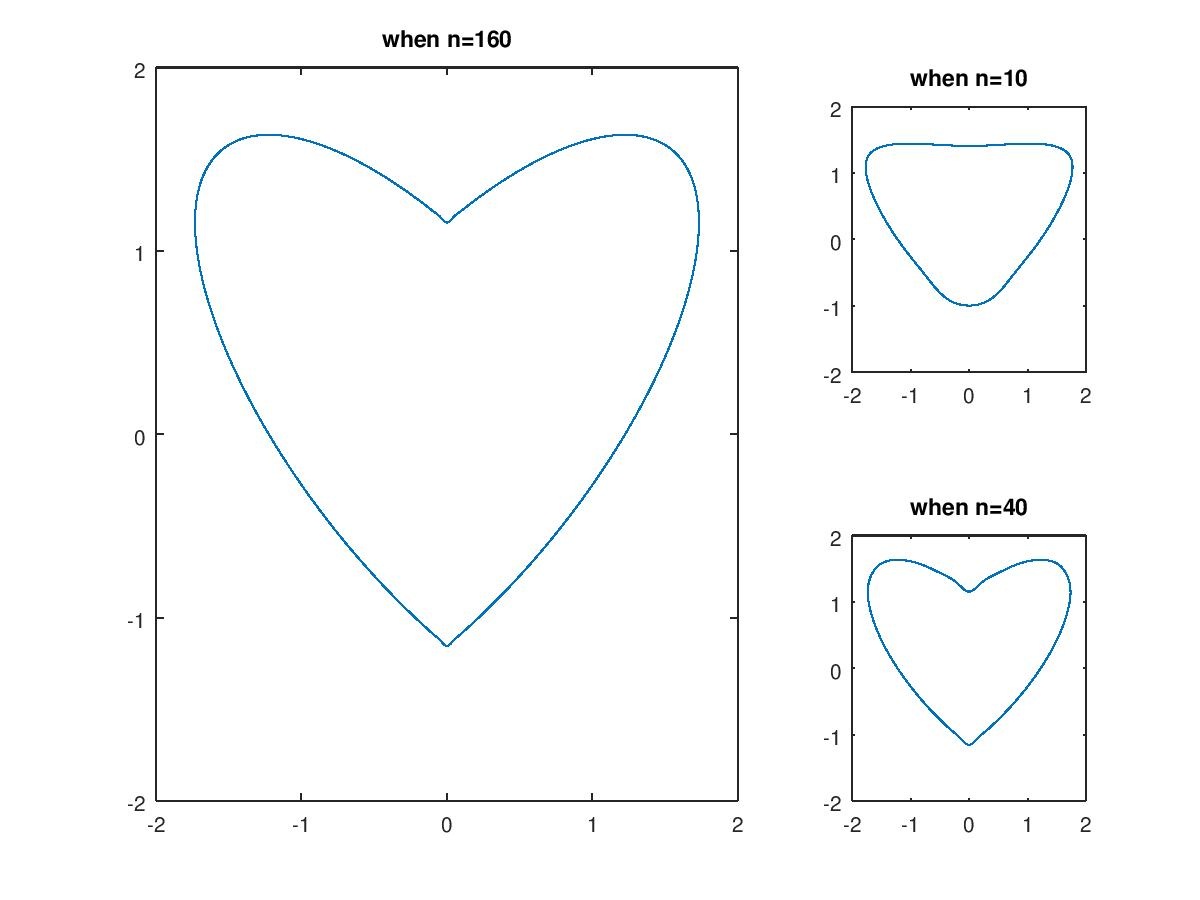
\includegraphics[width=14cm,height=8cm]{../plot/figure/figure_E.jpg}
\end{figure}

\subsection{Assignment.F}
\par 程序运行结果绘制出的图像如下:
\begin{figure}[H]
	\centering
	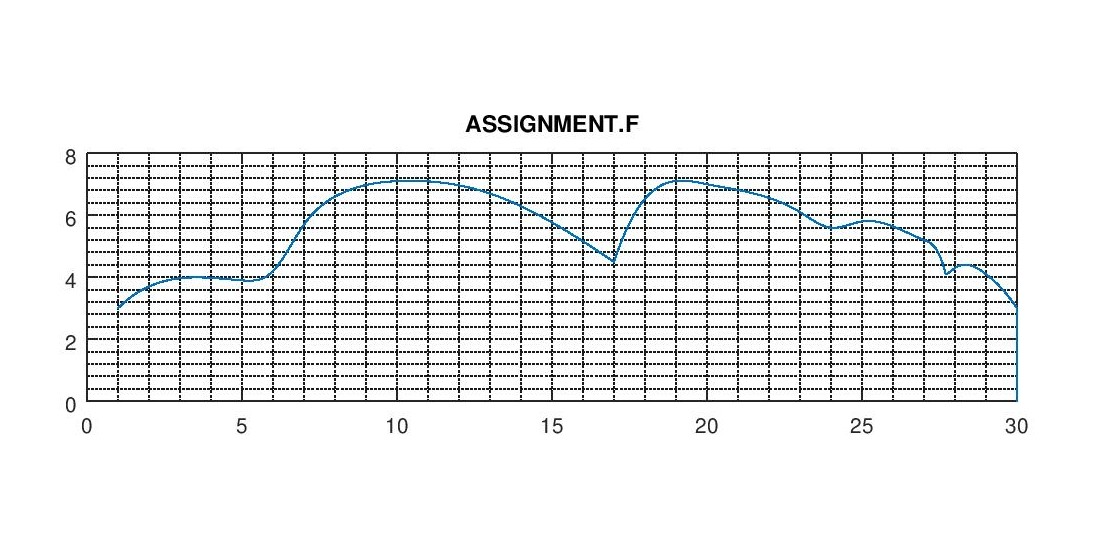
\includegraphics[width=0.85\textwidth]{../plot/figure/figure_F.jpg}
\end{figure}

\subsection{Assignment.G}
\begin{itemize}
	\item[(1)] n=1:
	\begin{figure}[H]
		\centering
		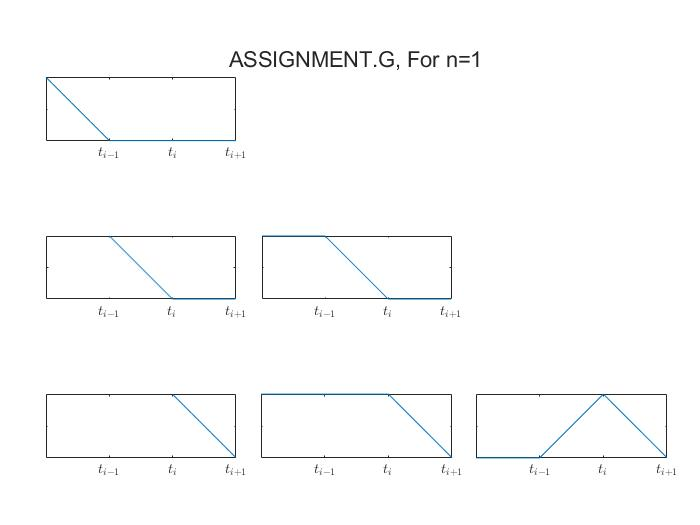
\includegraphics[scale=0.6]{../plot/figure/figure_G_1.jpg}
	\end{figure}
	\item[(2)] n=2:
	\begin{figure}[H]
		\centering
		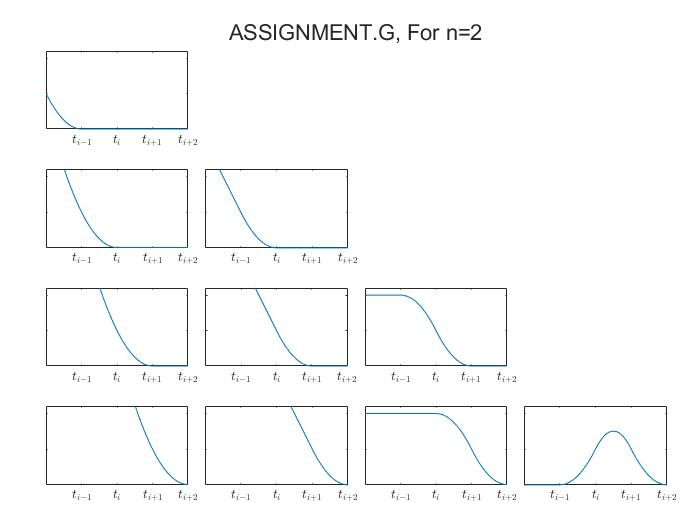
\includegraphics[scale=0.6]{../plot/figure/figure_G_2.jpg}
	\end{figure}
\end{itemize}

\end{large}
\end{document}